\documentclass{smilebeamer}

\mode<presentation> {
\usetheme{default}
}

\iffalse
\setbeamertemplate{footline}
{%
  \leavevmode%
  \hbox{\begin{beamercolorbox}[wd=.5\paperwidth,ht=2.5ex,dp=1.125ex,%
                              leftskip=.3cm plus1fill,rightskip=.3cm]%
                              {author in head/foot}%
  \usebeamerfont{author in head/foot}\ifnum\thepage=1\insertauthor\fi
  \end{beamercolorbox}%
  \begin{beamercolorbox}[wd=.5\paperwidth,ht=2.5ex,dp=1.125ex,leftskip=.3cm,%
    rightskip=.3cm plus1fil]{title in head/foot}%
    \usebeamerfont{title in head/foot}\insertshorttitle
  \end{beamercolorbox}}%
  \vskip0pt%
}
\fi

\setbeamertemplate{enumerate items}[default]
\usepackage{wasysym}
\usepackage{graphicx}
\usepackage{listings}
\usepackage{dirtytalk}
\usepackage{tikzsymbols}

\graphicspath{{img/}}

\lstset{basicstyle=\ttfamily\scriptsize}

\title[]{LLVM/Clang integration to Buildroot}

\author{Valentin Korenblit}
\iffalse
\institute[Smile]
{
Smile \\~\\
\medskip
\textit{valentin.korenblit@smile.fr}
}
\fi
\date{\today}

\begin{document}

\begin{frame}
\titlepage
\end{frame}

\begin{frame}
\frametitle{Overview}
\tableofcontents
\end{frame}

%-------------------------------------------------------
\section{Smile}

\begin{frame}
\frametitle{Smile - Open Source Solutions}
\begin{columns}[c]
\column{.5\textwidth}
\begin{itemize}
  \item 1st integrator and European expert in open source solutions
  \item Some numbers:
  \begin{itemize}
    \item 27 years of experience
    \item 1300 contributors
    \item 15 agencies in 7 countries
  \end{itemize}
\end{itemize}
\column{.5\textwidth}
\begin{figure}[H]
\centering
  
\includegraphics[scale=0.25]{img/smile_offers.png}
\end{figure}
\end{columns}
\end{frame}

%-------------------------------------------------------
\section{Internship objectives}

\begin{frame}
\frametitle{Internship objectives}
\begin{itemize}
  \item Preliminary study of LLVM/Clang
  \item LLVM/Clang integration to Buildroot
  \begin{itemize}
    \item llvmpipe for Mesa 3D
    \item AMDGPU backend
    \item OpenCL implementations
  \end{itemize}
  \item OpenCL support for already existing packages in Buildroot
  \item Integration of new packages that can benefit from OpenCL:
  image processing (i.e. Darktable), simulation, cryptography, etc.
\end{itemize}
\end{frame}
%-------------------------------------------------------
\section{LLVM}

\begin{frame}
\frametitle{LLVM}
\begin{itemize}
  \item Open source project started in 2000. LLVM 1.0 released in October 2003
  \begin{itemize}
    \item Several subprojects: LLVM Core, Clang, lldb, compiler-rt, libclc, lld
  \end{itemize}
  \item Provides a compiler infrastructure written in C++
  \begin{itemize}
    \item Designed as an API from the beginning
    \item Focusing on compile time and performance of the generated code
  \end{itemize}
  \item Well structured and documented
  \item Some existing backends:
  \begin{itemize}
    \item \textbf{ARM}, ARM64, Hexagon, Mips, Mipsel, NVIDIA PTX 32/64,
    PowerPC 32/64, \textbf{AMDGPU}, Sparc, Thumb, x86, \textbf{x86-64}, XCore
  \end{itemize}
\end{itemize}
\end{frame}

\begin{frame}
\frametitle{LLVM - Three-phase approach}
\begin{figure}
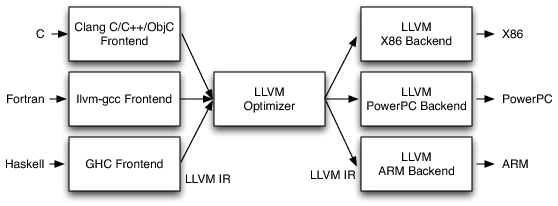
\includegraphics[width=1\linewidth]{img/llvm_struct.png}
\end{figure}
\end{frame}

\begin{frame}[fragile]
\frametitle{LLVM - Internal aspects}
\begin{itemize}
  \item Intermediate Representation (IR)
  \begin{itemize}
    \item Mostly architecture-independent instruction set (RISC)
    \item Strongly typed
    \item Unlimited number of virtual registers in SSA
  \end{itemize}
  \item IR Code example:
\end{itemize}

\begin{lstlisting}
      define i32 @main() #0 {
      entry:
        %retval = alloca i32, align 4
        %c = alloca i32, align 4
        store i32 0, i32* %retval, align 4
        %0 = load i32, i32* @a, align 4
        %1 = load i32, i32* @b, align 4
        %add = add nsw i32 %0, %1
        store i32 %add, i32* %c, align 4
        ret i32 0
      }
\end{lstlisting}
\end{frame}


%-------------------------------------------------------
\section{Clang}

\begin{frame}
\frametitle{Clang}
\begin{itemize}
  \item Frontend C/C++, Objective C/C++ and OpenCL C for LLVM
  \item Clear and concise diagnostics (error and warning messages)
  \item Natively a cross-compiler: {\fontfamily{qcr}\selectfont -target <triple>}
  \item Sanitizers
  \item Goals
  \begin{itemize}
    \item Designed to be highly compatible with GCC
    \item C++14 supported since Clang 3.4
    \item C++17 supported since Clang 5
  \end{itemize}
  \item Performance vs GCC ?\footnote{\url{http://www.phoronix.com/vr.php?view=25742}}
\end{itemize}
\end{frame}
%-------------------------------------------------------
\section{Who is using LLVM/Clang}

\begin{frame}
\frametitle{Who is using LLVM/Clang}
\begin{itemize}
  \item Android: Renderscript compiler based on LLVM
  \item Apple
  \begin{itemize}
    \item All operating systems built with Clang
    \item Xcode IDE uses Clang compiler and static analyzer by default
  \end{itemize}
  \item FreeBSD can be entirely built with Clang/LLVM
  \item Google is using Clang for building:
  \begin{itemize}
    \item Android user space
    \item Chrome for all platforms (since March 2018)
  \end{itemize}
  \item OpenCL: AMD, Apple, Intel, NVidia (runtime compiler)
  \item OpenJDK: Shark JIT compiler for Zero
  \item Sony Interactive Entretainment: CPU compiler for PS4
\end{itemize}
\end{frame}
%-------------------------------------------------------
\section{Compiling Linux with Clang}

\begin{frame}
\frametitle{Compiling Linux with Clang}
\begin{itemize}
  \item Challenges
  \begin{itemize}
    \item Linux kernel expects to use some GCC behavior that is not supported by Clang:
    \begin{itemize}
      \item Variable Length Arrays inside structures
      \item Nested functions
      \item Explicit register variables
      \item LLVM assembler cannot be used to build the kernel
    \end{itemize}
  \end{itemize}
  \item LLVMLinux Project: Kernel 4.4 and 4.9 built with Clang for x86\_64 and ARM64
  (patches applied)\footnote{https://lwn.net/Articles/734071/}
  \item Still depends on GNU {\fontfamily{qcr}\selectfont as} and {\fontfamily{qcr}\selectfont ld}
  \item glibc\footnote{https://sourceware.org/glibc/wiki/GlibcMeetsClang} ?
\end{itemize}
\end{frame}

%-------------------------------------------------------
\section{Toolchain components}
\begin{frame}
\frametitle{Toolchain components}
\centering
  \begin{tabular}{c|c|c}
  \textbf{Component} & \textbf{LLVM} & \textbf{GNU} \\
  \hline
  C/C++ Compiler & clang & gcc \\
  Assembler & cc1as & as \\
  Linker & lld & ld \\
  Runtime & compiler-rt & libgcc \\
  Debugger & lldb & gdb \\
  Unwinder & libunwind & libgcc\_s \\
  C++ library & libc++abi, libc++ & libsupc++ libstdc++ \\
  Tools & llvm-ar, llvm-as etc. & ar, objdump, etc. \\
  C library & - & libc \\
  \end{tabular}
\end{frame}

%-------------------------------------------------------
\section{LLVM/Clang integration to Buildroot}


\begin{frame}
\frametitle{LLVM/Clang integration to Buildroot - What does it enable?}
\begin{itemize}
  \item Gallium llvmpipe driver: software rasterizer that uses LLVM to do runtime code generation
  \begin{itemize}
    \item It is the fastest software rasterizer for Mesa3D
  \end{itemize}
  \item OpenSWR for scientific visualization (AVX, AVX2)
  \item Most OpenCL implementations rely on LLVM
\end{itemize}
\end{frame}



\begin{frame}
\frametitle{Project planning}
\begin{enumerate}
  \item Provide LLVM support for x86, ARM and AArch64
  \item Provide LLVM support for AMDGPU (R600 to GCN)
  \item Enable LLVM support for Mesa 3D:
    \begin{itemize}
      \item Gallium Drivers: llvmpipe, R600, RadeonSI
    \end{itemize}
  \item Add Clang
  \item Activate OpenCL
  \begin{itemize}
    \item AMD GPUs (Clover)
    \item Broadcom Videocore IV (VC4CL)
  \end{itemize}
\end{enumerate}
\end{frame}


\begin{frame}
\frametitle{Available hardware for testing}
\begin{itemize}
  \item Platform 1 - x86\_64 (HP ProBook)
  \begin{itemize}
    \item Processor: AMD A4-3300M Dual Core @ 1.9 GHz
    \item GPU: AMD Radeon Dual Graphics (HD6480G + HD7450M)
  \end{itemize}
  \item Platform 2 - ARM (Raspberry Pi 2 Model B)
  \begin{itemize}
    \item Processor: ARMv7 Cortex-A7 Quad Core @ 900 MHz
    \item GPU: Broadcom Videocore IV
  \end{itemize}
  \item Platform 3 - ARM/AArch64 (Raspberry Pi 3 Model B)
  \begin{itemize}
    \item Processor: ARMv8 Cortex-A53 Quad Core @ 1.2 GHz
    \item GPU: Broadcom Videocore IV
  \end{itemize}
\end{itemize}
\end{frame}


\begin{frame}
\frametitle{LLVM package - Directory Layout}
\begin{itemize}
  \item llvm/lib/ Most source files are here
  \begin{itemize}
    \item IR
    \item AsmParser
    \item Bitcode
    \item Transforms
    \item Target
  \end{itemize}
  \item llvm/tools/ Executables built out of the libraries \footnote{https://llvm.org/docs/CommandGuide/index.html}
  \begin{itemize}
    \item llvm-as
    \item \textbf{llvm-config}
    \item lli
    \item llc
    \item opt
  \end{itemize}
  \item llvm/utils/ Utilities for working with LLVM source code
  \begin{itemize}
    \item codegen-diff
    \item llvmgrep
    \item \textbf{TableGen}
  \end{itemize}
\end{itemize}
\end{frame}


\begin{frame}
\frametitle{LLVM package}
\begin{itemize}
  \item CMake-based project
  \begin{itemize}
    \item Buildroot provides a CMake infrastructure \smiley
  \end{itemize}
  \item Plenty of options, some with misleading names
  \begin{itemize}
    \item {\fontfamily{qcr}\selectfont LLVM\_TARGETS\_TO\_BUILD}
    \item {\fontfamily{qcr}\selectfont LLVM\_TARGET\_ARCH}
    \item {\fontfamily{qcr}\selectfont LLVM\_DEFAULT\_TARGET\_TRIPLE}
    \item {\fontfamily{qcr}\selectfont LLVM\_HOST\_TRIPLE}
  \end{itemize}
  \item Difficult to be cross-compiled
  \begin{itemize}
    \item At least llvm-tblgen must be compiled for the host first
    \item It requires a modern and fully-featured toolchain
  \end{itemize}
  \item Takes a lot of time to compile
\end{itemize}
\end{frame}

\begin{frame}
\frametitle{LLVM packaging for Buildroot}
\begin{itemize}
  \item LLVM 5.0.1 selected
  \item Only LLVM libraries are needed (libLLVM.so), no tools
  \item The main problem: \textbf{llvm-config} not giving the desired output
  \begin{itemize}
    \item It's a compiled program. Normally ''config'' programs are scripts.
    \item llvm-config compiled for the host must be installed to the target's
    sysroot.
    \item Some output depends on its location and some other is contained in the
    binary \Sey
  \end{itemize}
  \item \textbf{Solution:} do a full installation of LLVM for the host using the
  same\footnote{Tools are not built for the target} configuration options as for
  the target and link LLVM tools with libLLVM.
\end{itemize}
\end{frame}

\begin{frame}
\frametitle{LLVM support for Mesa 3D drivers}
\begin{itemize}
  \item Gallium llvmpipe: fastest software rasterizer for Mesa
  \begin{itemize}
    \item Uses LLVM to do runtime code generation
  \end{itemize}
  \item Gallium R600 and RadeonSI
  \begin{itemize}
    \item Both use AMDGPU LLVM backend
  \end{itemize}
    \item Some benchmarks:
\end{itemize}
\centering
  \begin{tabular}{c|c|c}
  \textbf{Gallium Driver} & \textbf{GLMark2} & \textbf{GLMark2-es2} \\
  \hline
  R600 on HD6480 & 156 & 156 \\
  softpipe on AMD A4-3300M & 3 & 3 \\
  softpipe on Cortex-A53 (32-bit) & - & 0 \\
  softpipe on Cortex-A53 (64-bit) & - & 0 \\
  llvmpipe on AMD A4-3300M & 47 & 52 \\
  llvmpipe on Cortex-A53 (32-bit) & - & 11 \\
  llvmpipe on Cortex-A53 (64-bit) & - & 13 \\
  \end{tabular}
\end{frame}


\begin{frame}
\frametitle{Selecting llvmpipe}
\begin{figure}
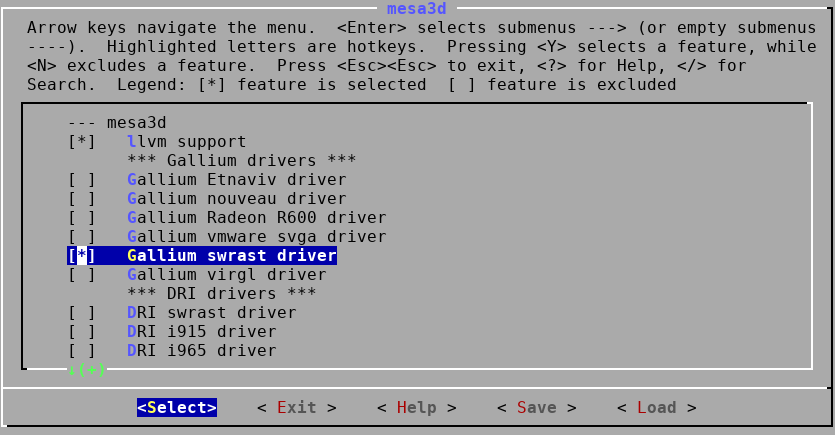
\includegraphics[width=1\linewidth]{img/mesa_swrast.png}
\end{figure}
\end{frame}


\begin{frame}
\frametitle{OpenCL}
\begin{itemize}
  \item API enabling general purpose computing on GPUs, CPUs, DSP,s FPGAs, etc.
  Well suited for certain kinds of parallel computations:
  \begin{itemize}
    \item Hash cracking (SHA, MD5, etc.)
    \item Image processing
    \item Simulations
  \end{itemize}
  \item OpenCL presents itself as a library with a simple interface:
  \begin{itemize}
    \item Standarized API headers for C and C++
    \item The OpenCL library (libOpenCL.so): collection of types and functions
    which all conforming implementations must provide.
  \end{itemize}
\end{itemize}
\end{frame}

\begin{frame}
\frametitle{OpenCL - Open Source Implementations}
\centering
{
\begin{tabular}{c|c|c}
\textbf{Project} & \textbf{Version} & \textbf{Hardware} \\
\hline
Clover & 1.1 & AMD\\
Pocl & 1.2 & CPU, NVIDIA\footnote{Needs propietary drivers}, AMD\footnote{HSA
compatible hardware}, TCE/TTA\\
Beignet & 2.0 & Intel\\
ROCm OpenCL & 1.2 & AMD\footnote{ROCm compatible hardware}\\
\end{tabular}
}
\vfill
\begin{itemize}
  \item OCL ICD Loader allows multiple OpenCL implementations to co-exist on
  the same system
\end{itemize}
\end{frame}

\begin{frame}
\frametitle{Clover}
\begin{figure}
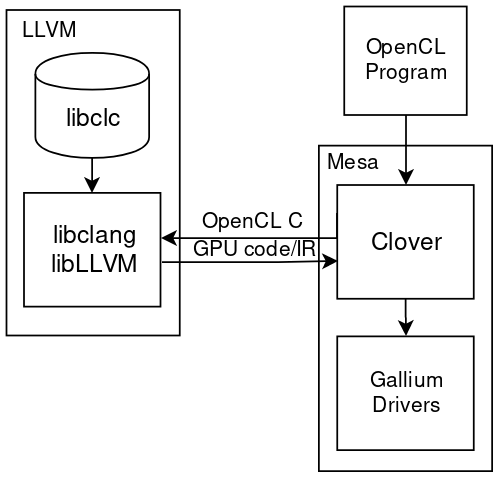
\includegraphics[width=0.7\linewidth]{img/clover.png}
\end{figure}
\end{frame}


\begin{frame}
\frametitle{Clang packaging for Buildroot}
\begin{itemize}
  \item host-clang is needed to compile libclc
  \begin{itemize}
    \item Many functions writen in LLVM IR (.ll)
  \end{itemize}
  \item It is normally built inside LLVM source tree (llvm/tools) but Buildroot
  uses per-package build directories.
  \begin{itemize}
    \item Some more tweaks are needed
  \end{itemize}
  \item Binaries, headers and some scripts must be removed from the target.
  \begin{itemize}
    \item Only libclang.so is necessary.
  \end{itemize}
\end{itemize}
\end{frame}



\begin{frame}
\frametitle{libclc packaging for Buildroot}
\begin{itemize}
  \item Builtin functions defined in the OpenCL 1.1 specification
  \begin{itemize}
    \item sin, cos, min, max, etc.
  \end{itemize}
  \item LLVM IR bitcode
  \item Also provides headers needed to compile OpenCL kernels by
  calling {\fontfamily{qcr}\selectfont clCreateProgramWithSource}
  \item Main problem: Buildroot removes {\fontfamily{qcr}\selectfont /usr/include}
  from the target filesystem
\end{itemize}
\end{frame}


\begin{frame}
\frametitle{Testing Clover: Piglit}
\begin{figure}
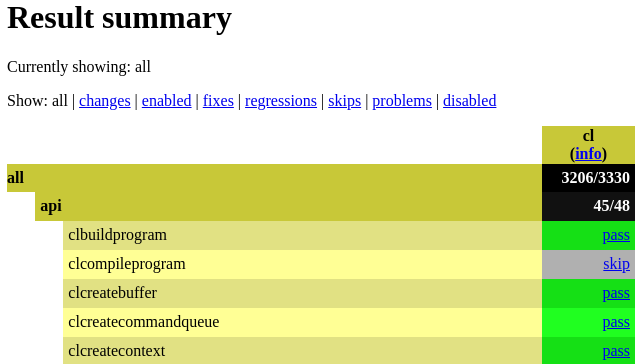
\includegraphics[width=0.9\linewidth]{img/html_output.png}
\end{figure}
\centering
\begin{tabular}{c|c|c|c|c}
Total & Skip & Pass & Fail & Crash \\
\hline
704 & \color{blue}{94} & \color{green}{541} & \color{red}{60} & 9
\end{tabular}
\end{frame}

\begin{frame}
\frametitle{Bonus: OpenCL for VideoCore IV (Raspberry Pi)}
\begin{itemize}
  \item VC4CL Project: OpenCL 1.2 EMBEDDED PROFILE
  \begin{itemize}
    \item VC4C: compiles OpenCL kernels into machine code.
    \item VC4CLStdLib: platform-specific implementation of the OpenCL C standard
    library.
  \end{itemize}
  \item VC4C calls Clang driver (binary) instead of linking against libclang.so
  \begin{itemize}
    \item Buildroot does not allow a compiler to be installed on the target
  \end{itemize}
  \item Kernel compilation is extremely slow on the target.\\
  \textbf{Solution:} compile kernels to LLVM IR bitcode on the host with host-clang and
  call {\fontfamily{qcr}\selectfont clCreateProgramWithBinary} instead of
  {\fontfamily{qcr}\selectfont clCreateProgramWithSource}
  \begin{itemize}
    \item Attention: code must be device-specific
  \end{itemize}
\end{itemize}
\end{frame}

\begin{frame}
\frametitle{LLVM/Clang for Buildroot - Current State}
\begin{itemize}
  \item Commited to Buildroot's master:
  \begin{itemize}
    \item LLVM package \checkmark
    \item LLVM support for Mesa 3D \checkmark
    \item Clang package \checkmark
  \end{itemize}
  \item Patchs sent to the mailing list:
  \begin{itemize}
    \item libclc package
    \item OpenCL support for AMD GPUs
  \end{itemize}
  \item TODO
  \begin{itemize}
    \item Add OpenCL support for already existing packages
    \item Add new packages that depend on LLVM
  \end{itemize}
\end{itemize}
\end{frame}

%-------------------------------------------------------
\begin{frame}
\Huge{\centerline{Questions?}}
\end{frame}

\end{document}
